\subsection{The Actor Model}
\label{actorModel}

In the same way that new programming languages embrace the multicore
nature of todays CPUs, I believe distributed programming
and the languages that are used to build highly distributed
systems should embrace the distributedness of the systems they
describe and should provide special syntax and semantics
for the unique problems inherent to the distributed systems domain
and there are ideas and languages that support this
view, as for example presented by Waldo et a. in \cite{noteondistributed}.
\newline

On the language side an alternative paradigm to programming
called the \textit{Actor Model} \cite{actors73}, \cite{actors2010}
has started to become widely adopted by the distributed systems
community and implemented by languages like
\textit{Erlang} \cite{erlang}, \cite{armstrongerlang} or
\textit{Pony} \cite{pony}.

Since its perception in 1973 by Hewitt et al. \cite{actors73},
the actor model has received a great amount of attention in the
academic community and has also been used to model concurrent
computation as an alternative to the threading model. It is therefor
also closely related to numerous process calculi like Hoare's
\textit{Communicating Sequential Processes} \cite{hoarecsp} and
the Milner's \textit{Pi Calculus} \cite{pimilner}.

Erlang is an actor based functional programming language
developed by Ericsson, a multinational telecommunications equipment
and services company and was designed to be used by their
telecommunications infrastructure.
\newline

\begin{wrapfigure}{r}{0.45\textwidth}
  \vspace{-10mm}
  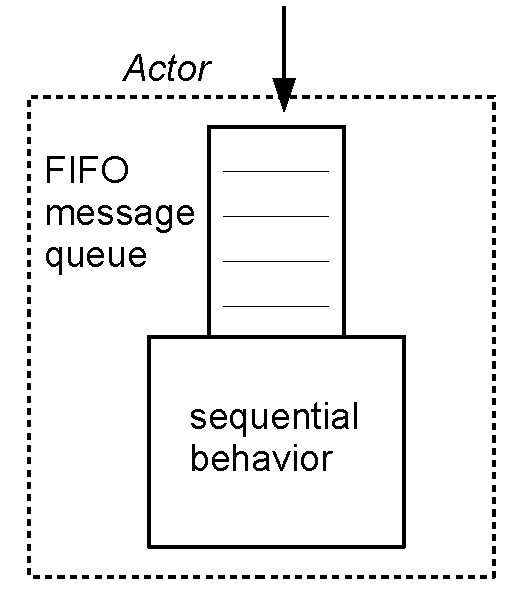
\includegraphics[width=0.4\textwidth]{actor.pdf}
  \caption{Concept of an \textit{Actor} as \\defined by the
          actor model.}
  \label{actor}
  \vspace{-25mm}
\end{wrapfigure}

The core concepts of the actor model as outlined in \cite{actorsagha}
and \cite{actors2010}
can be summarized as follows. The actor model treats \textit{actors}
(or processes) as its universal primitives of computation.
These actors are autonomous in the sense that each actors executed
behavior is independent of the concurrent existence of other actors.
However, in order to interact with others, actors can send and receive
messages as illustrated in Fig.\ref{actor}. So each actor consists
of its single threaded behavior and a single input message queue.

The actor can now decide whether or not and how to react to
its incoming messages and can also send messages directly to other
actors. Its behavior itself though is single threaded.
The concurrent nature of an actor based system lies within the
actor model itself because of the actors being executed independent
of each other.

This also means that the only means of communication,
namely message passing, is \textit{asynchronous} by default.
The actor model iself does not define any receipt or acknowledgement mechanism
for messages received by an actors input queue. Any such communication
protocol must be implemented by the actors themselves, e.g. by
programming their behavior to send an acklowdgement to the sender once
a message is processed. This means that, using the plain actor model,
a sender cannot only not infer whether or not its message was processed
or perceived by its receiver, it can't even infer whether or not
the message ever reached the receiver.
\newline

This seems ludicrous compared to the implicit safety and messaging
guarantees promised by the \textit{distributed objects} approach
presented in chapter \ref{DistributedObjects} where synchronous
messaging is as \textit{easy} as a local function call. But this
seemingly pessimistic approach to messaging turns out to be
acceptably close that what must be anticipated when dealing with
messaging in highly distributed systems on the data center and cloud
scale.

So again the actor model seems to provide a sweetspot because on
the one hand it encompasses characteristic properties of highly
distributed systems, i.e. virtually no message delivery guarantees,
thereby forcing the developer to deal with these circumstances
in her program structure and application design and on the other
hand provides small, independent and single threaded units of
computation in order to build more abstract and higher level
distributed applications.

\setlength{\intextsep}{10pt}
\setlength{\columnsep}{20pt}

\begin{wrapfigure}{l}{0.5\textwidth}
    \begin{lstlisting}
-module (send_recv).
-compile([export_all]).

serve() ->
  receive
    Request ->
      io:format("received request~n"),
      serve()
  end.

run() ->
  Pid = spawn(?MODULE, serve, []),
  Pid ! Request,
  ok.
    \end{lstlisting}
  \caption{Erlang example of how to spawn an Actor using the \textit{spawn}
          function and how to use the messaging operator \textit{!}}
  \label{erlang-example}
  \vspace{-20mm}
\end{wrapfigure}

Since Erlang is an actor based language, Fig.\ref{erlang-example}
shows a small example. It spawns an actor executing the
user-defined \textit{serve()} function. Spawning an actor is done
using the built-in \textit{spawn()} function. The serve() function
contains a \textit{receive-loop}, another Erlang built-in indicated
by the \textit{receive} keyword. This loop listens for incoming
messages and tries to match any incoming message to any of the
given patterns. So it can be thought of as the combination of an
implicit event loop and a switch-case statement.

In the case of this example any message that consists of only a single
atom will be matched to the user-defined Request pattern, triggering
a simple console print and a recursive call to restart the receive
loop. This is important because when the receive loop is entered it
will wait for incoming messages indefinitely unless a timeout is
specified. When a message arrives at the inbox that can be matched
against one of the provided patterns it will be processed as
programmed. When there are multiple messages in the actors inbox
that could be matched against some provided pattern only one
of them is being process and it is up to the actor when to
reenter the receive loop in order to process the remaining messages.

To address the actor or process created by the call to \textit{spawn()}
a process identifier (PID) is returned by spawn, which is the only
way to attain such an identifier. In order to send messages to this
PID Erlang provides the messaging operator \textit{'!'}.

This shows that message passing is an integral part of the core
language, including its pessimistic delivery guarantees (none), and
specified by the language itself. These semantics are therefor
not loosely defined in some library documentation that could
change any minute but are guaranteed to the programmer,
independent of the language implementation or execution environment.
\newline

Unfortunately there is a down side to this approach. Since the
actor model focusses so heavily on its actors, the result is that
the actual description of the system happens implicitely and
indirectly. It is more like the system \textit{emerges} out of all the
little steps and interactions of its components. To the effect that,
given a running system of maybe a hundred or a thousand actors
\cite{uber}, how would one come to understand what the system as
a whole is doing?

There is no other option than to just pick any actor and start
reading its code. This means one is forced to reverse engineer the
behavior of the entire system from the internal behavior of its parts
which, needless to say, can be quite error prone and introduces
nontrivial cognitive overhead. In other words, there is no way to
take a look at the system from the birds-eye perspective because
most people believe this implies introducing some form of global
state which would be against any of the goals of the actor model
with its asynchronous message passing and independent processes.
